%% LyX 2.3.6.2 created this file.  For more info, see http://www.lyx.org/.
%% Do not edit unless you really know what you are doing.
\documentclass[english]{beamer}
\usepackage{mathpazo}
\renewcommand{\sfdefault}{lmss}
\usepackage[T1]{fontenc}
\usepackage[latin9]{inputenc}
\usepackage{amssymb}
\usepackage{graphicx}

\makeatletter
%%%%%%%%%%%%%%%%%%%%%%%%%%%%%% Textclass specific LaTeX commands.
% this default might be overridden by plain title style
\newcommand\makebeamertitle{\frame{\maketitle}}%
% (ERT) argument for the TOC
\AtBeginDocument{%
  \let\origtableofcontents=\tableofcontents
  \def\tableofcontents{\@ifnextchar[{\origtableofcontents}{\gobbletableofcontents}}
  \def\gobbletableofcontents#1{\origtableofcontents}
}

%%%%%%%%%%%%%%%%%%%%%%%%%%%%%% User specified LaTeX commands.
\usetheme{Darmstadt}
%\usetheme{CambridgeUS}
% or ...

\setbeamercovered{transparent}
\setbeamertemplate{theorems}[numbered] 

\newcommand{\R}{\mathbb{R}}%
\newcommand{\T}{\mathcal{T}}%
\newcommand{\parens}[1]{\left(#1 \right)}%
\newcommand{\braces}[1]{\left\{#1 \right\}}%
\newcommand{\angles}[1]{\langle #1 \rangle}%
\newcommand{\dd}[1]{\frac{\d}{\d #1}}%
\newcommand{\ddd}[2]{\frac{\d #1}{\d #2}}%
\newcommand{\pd}[1]{\frac{\partial}{\partial #1}}%
\newcommand{\pdd}[2]{\frac{\partial #1}{\partial #2}}%
\newcommand{\evalat}[1]{\Big|_{#1}}%
\DeclareMathOperator*{\argmax}{argmax}%
\DeclareMathOperator*{\argmin}{argmin}%
\newcommand{\E}[1]{\text{E}\left[ #1 \right]}%
\newcommand{\bm}[1]{\boldsymbol{#1}}%

\makeatother

\usepackage{babel}
\begin{document}
\title{Non-linear protocols for optimal distributed consensus in networks
of dynamic agents}

\makebeamertitle

\pgfdeclareimage[height=0.5cm]{institution-logo}{uchicago_logo.jpeg}

%\logo{\pgfuseimage{institution-logo}}


\AtBeginSubsection[]{
  \frame<beamer>{ 
    %\frametitle{Outline}   
    \tableofcontents[currentsection,currentsubsection] 
  }
}
\AtBeginSection[]{
  \frame<beamer>{ 
    \frametitle{Outline}   
    \tableofcontents[currentsection] 
  }
}

%\beamerdefaultoverlayspecification{<+->}
\begin{frame}{TLDR...}

\begin{figure}
\centering{}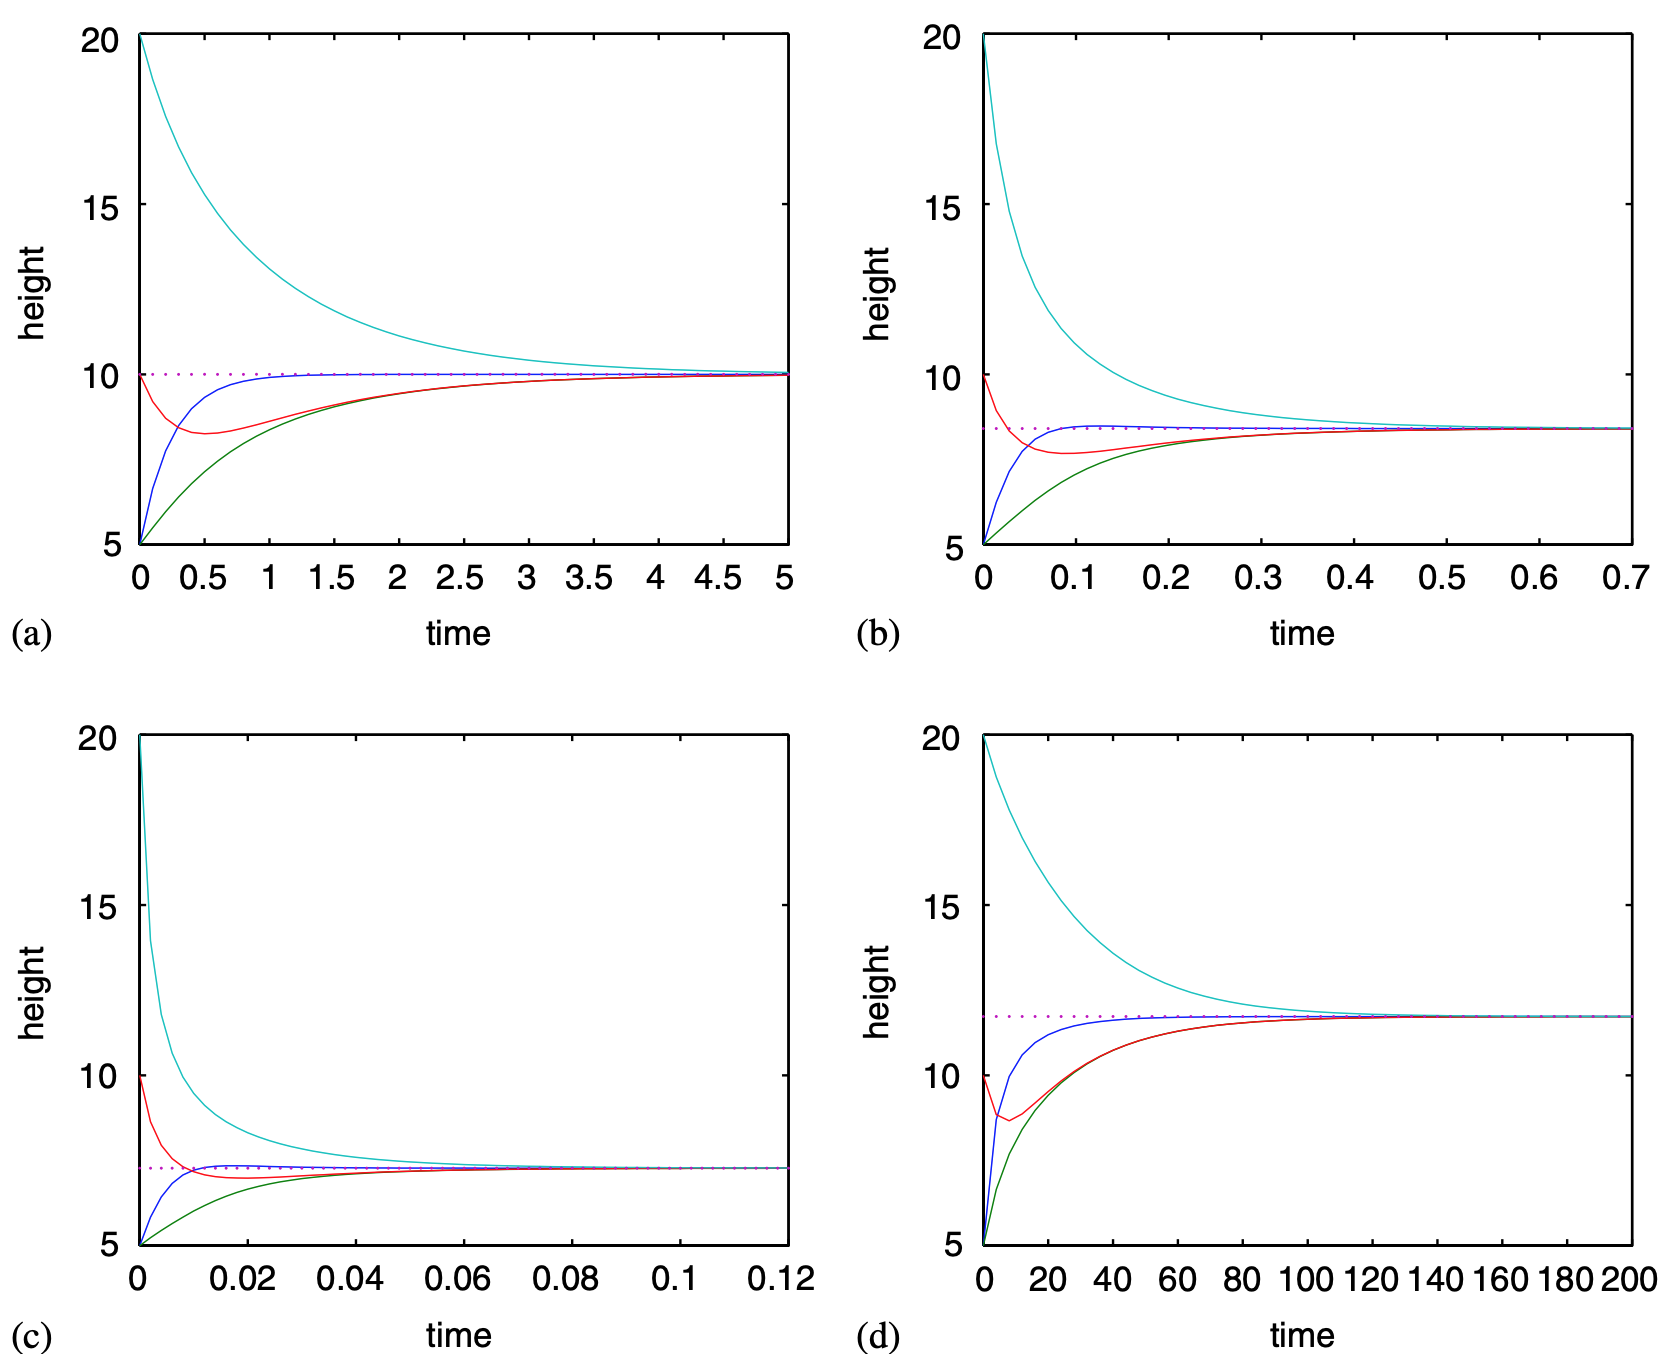
\includegraphics[width=0.75\linewidth]{tldr}
\end{figure}

\end{frame}

\begin{frame}{Outline}

\tableofcontents{}

\end{frame}

\section{Definitions}

\framesubtitle{}
\begin{frame}{}
\begin{block}<1->{Agents}
$\Gamma={1,\dots,n}$ is a set of \textit{agents/players/nodes/vertices}
and $G=(\Gamma,E)$ is a fixed (in time) undirected, connected, network
describing the connections between vertices $i\in\Gamma$, where $E\subset\Gamma\times\Gamma$
is the edge set. 
\end{block}

\pause{}

\begin{block}<2->{Neighborhood}
A \textit{neighborhood} of a vertex $i$ is the set of all vertices
$j$ for which there is a single edge connecting $i,j$, that is to
say $N_{i}:=\left\{ j\mid(i,j)\in E\right\} $.

\end{block}

\pause{}

\end{frame}

\begin{frame}{}
\begin{figure}
\begin{centering}
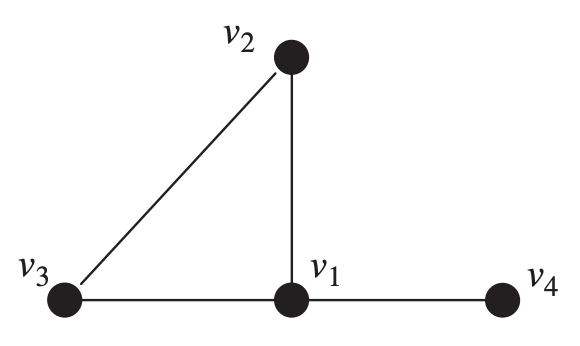
\includegraphics[width=0.5\linewidth]{neighbors1}\,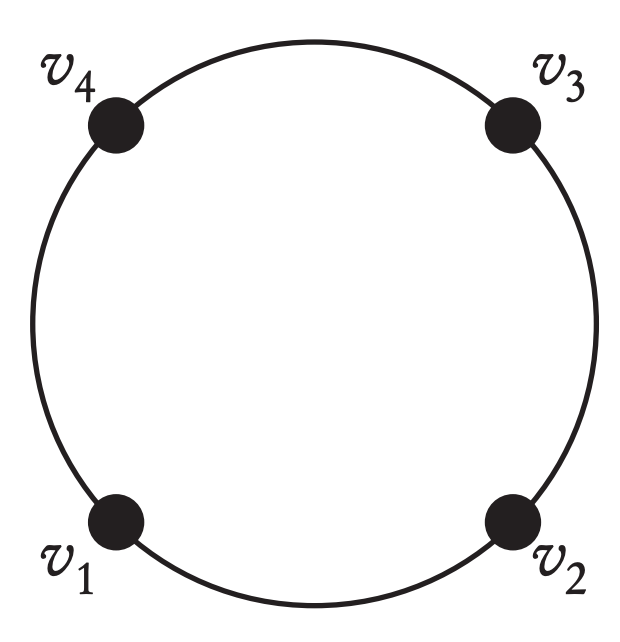
\includegraphics[width=0.33\linewidth]{neighbors2}\caption{Neighborhoods}
\par\end{centering}
\end{figure}
\end{frame}
%
\begin{frame}{}
\begin{block}{Control policy}
Let $x_{i}(t)$ be the state of the agent $i$ at time $t$, then
$x_{i}$ evolves according to a \textit{distributed} and \textit{stationary}
control policy $u_{i}$, if $\dot{x}_{i}=u_{i}(x_{i},\mathbf{x}_{N_{i}})$,
where $\mathbf{x}_{N_{i}}$ are the states of $x_{i}$'s neighbors. 

\end{block}

\pause{}
\begin{block}{Protocol}
The \textit{protocol} of the network is the collection of controls
$\vec{u}(\vec{x}):=(u_{i}(x_{i},\mathbf{x}_{N_{i}}))$ for all $i\in\Gamma$.
\end{block}
\end{frame}

\begin{frame}{}
\begin{block}{Agreement function}
The \textit{agreement function} $\chi:\R^{n}\rightarrow\R$ is any
continuous, differentiable function which is permutation invariant,
i.e.
\[
\chi(x_{1},\dots,x_{n})=\chi(x_{\sigma(1)},\dots,x_{\sigma(n)})
\]
\end{block}

\pause{}
\begin{block}{Consensus}
To \textit{reach consensus} on \textit{consensus value} $\chi(\mathbf{x}(0))$
means 
\[
\lim_{t\rightarrow\infty}\mathbf{x}(t)=\chi(\mathbf{x}(0))\mathbf{1}
\]
 where $\mathbf{1}:=(1,1,\dots,1)$.
\end{block}
\end{frame}

\section{The consensus problem}
\begin{frame}{}

\begin{block}{Consensus problem}
Given a network $G$ of agents and agreement function $\chi$, the
\textit{consensus problem} is to design a protocol $\mathbf{u}$ such
that consensus is reached for any consensus value $\chi(\mathbf{x}(0))$.
\end{block}

\pause{}
\begin{block}{Consensus protocol}
A protocol is a \textit{consensus protocol} if it is the solution
to a consensus problem. 
\end{block}
\end{frame}

\subsection{Time-invariance of $\chi$}
\begin{frame}
\begin{lemma}
Let $\mathbf{u}$ be a stationary consensus protocol. Then $\chi(\mathbf{x}(t))$
is stationary, i.e. $\chi(\mathbf{x}(t))=\chi(\mathbf{x}(0))$ for
all $t>0$.
\end{lemma}


\pause{}
\begin{proof}
By assumption $\mathbf{x}(t)\rightarrow\chi(\mathbf{x}(0))\mathbf{1}$.
Stationary $\mathbf{u}$ is equivalent to autonomous and therefore,
if $\mathbf{x}(t)$ is a solution, then $\mathbf{y}_{s}(t):=\mathbf{x}(t+s)$
(with $\mathbf{y}_{s}(0):=\mathbf{x}(s)$) is also a solution. For
such $\mathbf{y}_{s}$ we also have $\mathbf{y}_{s}(t)\rightarrow\chi(\mathbf{y}_{s}(0))\mathbf{1}$
i.e.
\[
\lim_{t\rightarrow\infty}\mathbf{y}_{s}(t)=\chi(\mathbf{y}_{s}(0)\mathbf{1})=\chi(\mathbf{x}(s))
\]
But since both $\mathbf{y}_{s},\mathbf{x}$ converge to the same limit
we must have $\chi(\mathbf{x}(s))=\chi(\mathbf{x}(0))$ for all $s$.
\end{proof}

\end{frame}
%

\subsection{Properties of $\mathbf{u}$}
\begin{frame}{}

\begin{example}<1->
On first slide. 
\end{example}

\begin{example}<2->
On second slide.
\end{example}

\end{frame}

\section{Our Results/Contribution}

\subsection{Main Results}
\begin{frame}{}

\begin{theorem}
On first slide.
\end{theorem}


\pause{}
\begin{corollary}
On second slide.
\end{corollary}

\end{frame}

\begin{frame}{}

\begin{columns}[t]


\column{5cm}
\begin{theorem}<1->
In left column.
\end{theorem}


\column{5cm}
\begin{corollary}<2->
In right column.\\
New line
\end{corollary}

\end{columns}

\end{frame}

\subsection{Basic Ideas for Proofs/Implementations}

\section*{Summary}
\begin{frame}{}

\begin{itemize}
\item The \textcolor{red}{first main message} of your talk in one or two
lines.
\item The \textcolor{red}{second main message} of your talk in one or two
lines.
\item Perhaps a \textcolor{red}{third message}, but not more than that.
\end{itemize}

\vskip0pt plus.5fill
\begin{itemize}
\item Outlook

\begin{itemize}
\item What we have not done yet.
\item Even more stuff.
\end{itemize}
\end{itemize}
\end{frame}

\appendix

\section*{Appendix}

\subsection*{For Further Reading}
\begin{frame}[allowframebreaks]{}

\beamertemplatebookbibitems
\begin{thebibliography}{References}
\bibitem{Author1990}A. Author. \newblock\emph{Handbook of Everything}.\newblock
Some Press, 1990.\beamertemplatearticlebibitems

\bibitem{Someone2002}S. Someone.\newblock On this and that\emph{.}
\newblock\emph{Journal on This and That}. 2(1):50--100, 2000.
\end{thebibliography}
\end{frame}

\end{document}
